\documentclass[border=2mm]{standalone}
\usepackage{tikz}
\usetikzlibrary{arrows,shapes,snakes,automata,backgrounds,petri,matrix}

\begin{document}
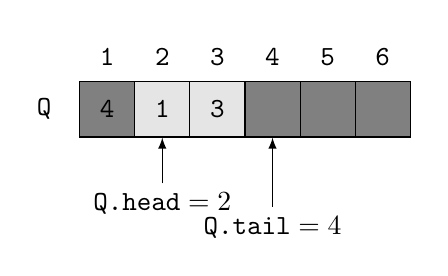
\begin{tikzpicture}[
font=\ttfamily, array/.style={
    matrix of nodes, 
    nodes={draw=black, minimum size=7mm, fill=gray, anchor=center},
    column sep=-\pgflinewidth, 
    row sep=0.5mm, 
    nodes in empty cells,
    row 1/.style={ nodes={draw=white, fill=none, minimum size=5mm}},
    row 1 column 1/.style={nodes={draw}},
},
]

\matrix[array] (array) {
   1  &  2  &  3  &  4  &  5  & 6\\
  4 &|[fill=gray!20]|1  &|[fill=gray!20]| 3  &  & & \\
};

\node (Q) [left of=array-2-1, node distance=0.8cm] {Q};
\node (T) [below of=array-2-4, node distance=1.5cm] {$\texttt{Q.tail}=4$};
\node (H) [below of=array-2-2, node distance=1.2cm, xshift=0cm] {$\texttt{Q.head}=2$};
\draw[-latex] (T) to (array-2-4);
\draw[-latex] (H) to (array-2-2);

\end{tikzpicture}
\end{document}
